\documentclass[12pt, a4paper, oneside]{Thesis} % Paper size, default font size and one-sided paper
\usepackage{wrapfig}
\usepackage{lscape}
\usepackage{rotating}
\usepackage{graphicx}
\usepackage{caption}
\usepackage{amsmath}
\usepackage{fancyhdr}
\usepackage[T1]{fontenc}
\usepackage{sectsty}

% prints author names as small caps

%\usepackage{subcaption} %incompatible with subfig
\graphicspath{{Pictures/}} % Specifies the directory where pictures are stored
\usepackage[square, numbers]{natbib} % Use the natbib reference package - read up on this to edit the reference style; if you want text (e.g. Smith et al., 2012) for the in-text references (instead of numbers), remove 'numbers' v

\hypersetup{urlcolor=black, colorlinks=true} % Colors hyperlinks in blue - change to black if annoyingv`	
\title{\ttitle} % Defines the thesis title - don't touch this

\begin{document}
% prints author names as small caps

\frontmatter % Use roman page numbering style (i, ii, iii, iv...) for the pre-content pages
\setstretch{1.5} % Line spacing of 1.6 (double line spacing)

% Define the page headers using the FancyHdr package and set up for one-sided printing
\fancyhead{} % Clears all page headers and footers

%\rhead{\thepage} % Sets the right side header to show the page number
%\lhead{} % Clears the left side page header

\pagestyle{fancy} % Finally, use the "fancy" page style to implement the FancyHdr headers

\newcommand{\HRule}{\rule{\linewidth}{0.4mm}} % New command to make the lines in the title page

% PDF meta-data
\hypersetup{pdftitle={\ttitle}}
\hypersetup{pdfsubject=\subjectname}
\hypersetup{pdfauthor=\authornames}
\hypersetup{pdfkeywords=\keywordnames}

%----------------------------------------------------------------------------------------
%	TITLE PAGE
%----------------------------------------------------------------------------------------

\begin{titlepage}
\begin{center}

%\HRule \\[0.4cm] % Horizontal line
{\huge \bfseries \ttitle{Project Title}}\\[0.10cm] % Thesis title
%\HRule \\[0.5cm] % Horizontal line
 
\large \textit{Submitted in partial fulfillment of the requirements \\ for the degree of \\ Bachelor of Engineering}\\[0.03cm] % University requirement text
\textit{by}\\[0.03cm]
\textbf{jayanth timmala}\\[0.01cm]
\textbf{Roll No.}\\[0.05cm]
\textbf{Name of the Student}\\[0.01cm]
\textbf{Roll No.}\\[0.05cm]
\textbf{Name of the Student}\\[0.01cm]
\textbf{Roll No.}\\[0.05cm]
\textit{Guide}\\[0.01cm] 
\textbf{Name of Guide}\\[0.35cm]
\begin{figure}[hb!]
 \centering
 
\includegraphics[scale=0.9]{Pictures/kgce_logo.png}
 % kgce_logo.png: 614x618 px, 300dpi, 5.20x5.23 cm, bb=0 0 147 148
\end{figure}
%\DEPTNAME\\ % Research group name and department name
\textsc{DEPARTMENT OF INFORMATION TECHNOLOGY \\[0.01cm]
KONKAN GYANPEETH COLLEGE OF ENGINEERING KARJAT-410201}\\[0.01cm] % University name
2024-25
\end{center}

\end{titlepage}

%----------------------------------------------------------------------------------------
%	DECLARATION PAGE
%	Your institution may give you a different text to place here
%----------------------------------------------------------------------------------------
\clearpage % Start a new page
%\raisebox{0.0\height}[0pt][0pt]{
\includegraphics[width=0.99\textwidth]{Pictures/KGCE_Letter_head_header.png}}
\Declaration{
\addtocontents{toc}{\vspace{0.8em}} % Add a gap in the Contents, for aesthetics
This is to certify that the project entitled \textbf{"Title of project"} is a bonafide work of\newline
\begin{enumerate}
    \item \textbf{Student Name} \textbf{Roll Number}
    \item \textbf{Student Name} \textbf{Roll Number}
    \item \textbf{Student Name} \textbf{Roll Number}
    \item \textbf{Student Name} \textbf{Roll Number}
\end{enumerate}

submitted to the University of Mumbai in partial fulfillment of the requirement for the award of the degree of \textbf{Bachelor of Engineering} in \textbf{Department of Information Technology Engineering} during academic year 2024-25. \\

\begin{minipage}{0.5\textwidth}
	\begin{flushleft} %\large
		%\emph{\large \today}\\[2cm] % Date
	\end{flushleft}
\end{minipage}
\begin{minipage}{0.5\textwidth}
	{\begin{center} \large
		\textbf{Guide}
		\begin{center}
			{\textlangle name\textrangle \\ 
			\normalsize{Department of Information Technology Engineering}}
		\end{center}
	\end{center}}
\end{minipage} \\[2.0cm]

\begin{minipage}{0.5\textwidth}
	\begin{flushleft} 
		{\begin{center} \large
		\textbf{Head of Department}
		\begin{center}
			{\textlangle name\textrangle \\ 
			\normalsize{Department of AI \& data Science}}
		\end{center}
	\end{center}}
	\end{flushleft}
\end{minipage}
\begin{minipage}{0.5\textwidth}
	{\begin{center} \large
		\textbf{Principal}
		\begin{center}
			{Dr. Vilas Janardan Pillewan\\ 
			\normalsize{Konkan Gyanpeeth College of Engineering, Karjat}}
		\end{center}
	\end{center}}
\end{minipage}
 %\raisebox{-3.8\height}[0pt][0pt]{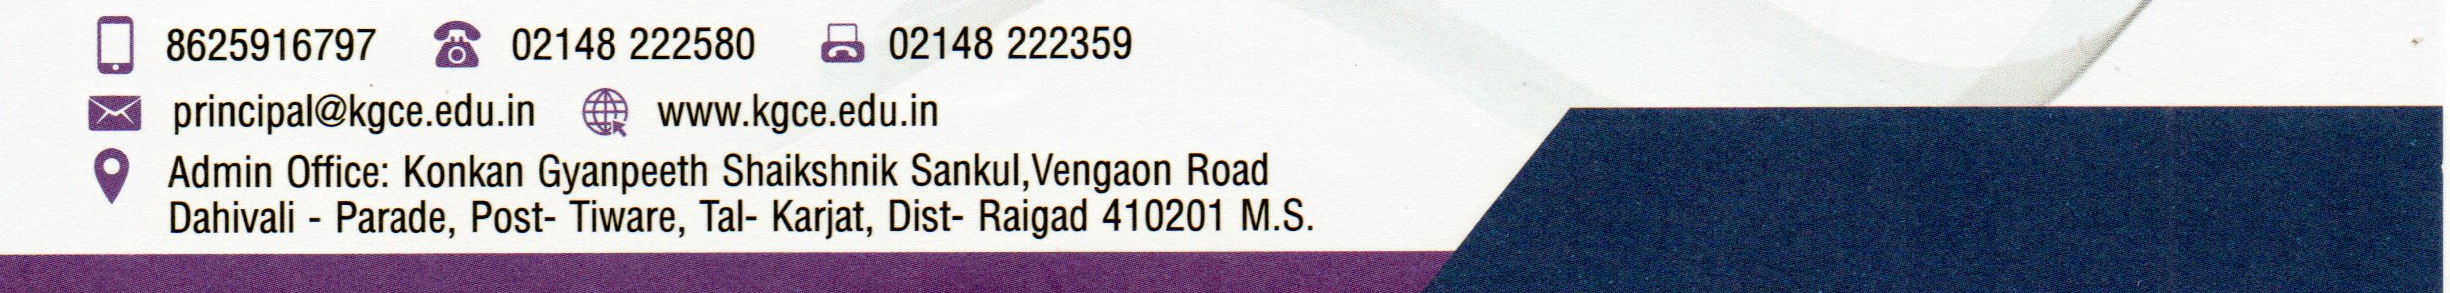
\includegraphics[width=\textwidth]{Pictures/KGCE_Letter_head_footer.png}} 
}
%----------------------------------------------------------------------------------------
%	DECLARATION PAGE
%	Your institution may give you a different text to place here
%----------------------------------------------------------------------------------------

\clearpage % Start a new page
%\raisebox{0.0\height}[0pt][0pt]{
\includegraphics[width=0.99\textwidth]{Pictures/KGCE_Letter_head_header.png}}

\Declarationa{\addtocontents{toc}{\vspace{1em}} % Add a gap in the Contents, for aesthetics
This report entitled \textbf{"Project Title"} submitted by\\
\begin{enumerate}
    \item \textbf{Student Name} \textbf{Roll Number}
    \item \textbf{Student Name} \textbf{Roll Number}
    \item \textbf{Student Name} \textbf{Roll Number}
    \item \textbf{Student Name} \textbf{Roll Number}
\end{enumerate}
is approved for the degree of Bachelor of Engineering in \textbf{Information Technology Engineering} during academic year 2024-25. \\[1cm]

\begin{minipage}{0.5\textwidth}
	\begin{flushleft} %
	
		%\emph{\large \today}\\[2cm] % Date
	\end{flushleft}
\end{minipage}
\begin{minipage}{0.5\textwidth}
	{\begin{center} \large
		\textbf{Examiners}\\[2cm]
		\begin{center}
			{1..........................................\\[2.25cm]
			2..........................................}
		\end{center}
	\end{center}}
\end{minipage} \\[1.5cm]
\large\textbf{Date: \\ Place:}
%\raisebox{-3.5\height}[0pt][0pt]{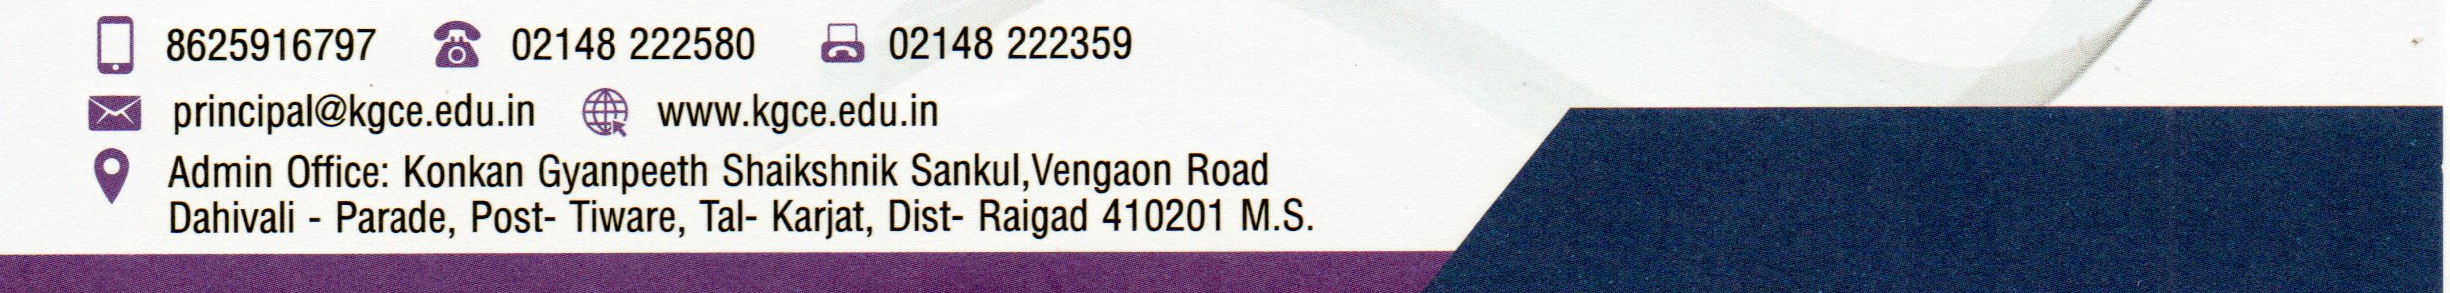
\includegraphics[width=\textwidth]{Pictures/KGCE_Letter_head_footer.png}}
}

%----------------------------------------------------------------------------------------
%	DECLARATION PAGE
%	Your institution may give you a different text to place here
%----------------------------------------------------------------------------------------
\clearpage % Start a new page
%\raisebox{0.0\height}[0pt][0pt]{
\includegraphics[width=0.99\textwidth]{Pictures/KGCE_Letter_head_header.png}}
%\vspace{15mm}
\Declarationb{\addtocontents{toc}{\vspace{1em}} % Add a gap in the Contents, for aesthetics
We declare that this written submission represents my ideas in my own words and where others' ideas or words have been included, We have adequately cited and referenced the original sources. We also declare that we have adhered to all principles of academic honesty and integrity and have not misrepresented or fabricated or falsified any idea/data/fact/source in our submission. We understand that any violation of the above will be cause for disciplinary action by the Institute and can also evoke penal action from the sources which have thus not been properly cited or from whom proper permission has not been taken when needed.\\[1cm]

\begin{minipage}{0.5\textwidth}
	\begin{flushleft} %\large
		%\emph{\large \today}\\[2cm] % Date
	\end{flushleft}
\end{minipage}
\begin{minipage}{0.5\textwidth}
	{\begin{center} \large
		\textbf{Signature}\\
		\textbf{(Name of Student) Roll No}\\[1cm]
		\textbf{Signature}\\
		\textbf{(Name of Student)  Roll No}\\[1cm]
		\textbf{Signature}\\
		\textbf{(Name of Student)  Roll No}\\[1cm]
		\textbf{Signature}\\
		\textbf{(Name of Student)  Roll No}
	\end{center}}
 
\end{minipage} \\[1cm]
  \large\textbf{Date: \\ Place:}
  %\raisebox{-2.3\height}[0pt][0pt]{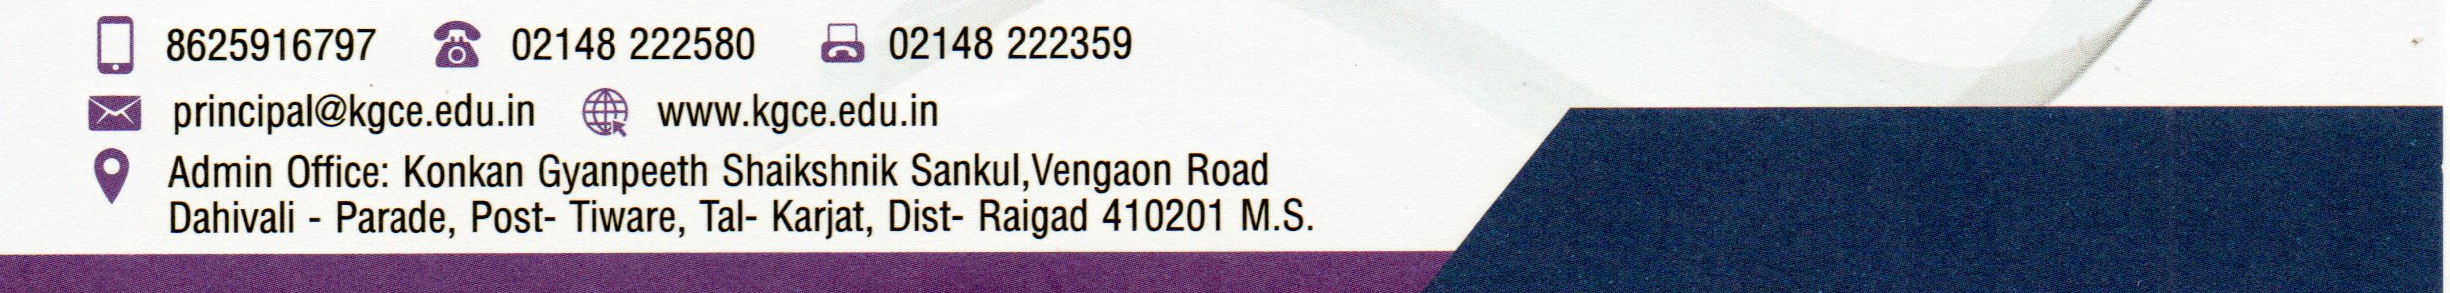
\includegraphics[width=\textwidth]{Pictures/KGCE_Letter_head_footer.png}} 
}

\clearpage % Start a new page
%----------------------------------------------------------------------------------------
%	ABSTRACT PAGE
%----------------------------------------------------------------------------------------

\addtotoc{Abstract} % Add the "Abstract" page entry to the Contents

\abstract{\addtocontents{toc}{\vspace{1em}} % Add a gap in the Contents, for aesthetics

Enter Abstract Content here.........This should be one/two short paragraphs (100-150 words total), summarizing the project work. It is important that this is not just a re-statement of the original project outline. A suggested flow is background, project aims and main achievements. From the abstract, a reader should be able to ascertain if the project is of interest to them and, it should present results of which they may wish to know more details.
}

\clearpage % Start a new page

%----------------------------------------------------------------------------------------
%	LIST OF CONTENTS/FIGURES/TABLES PAGES
%----------------------------------------------------------------------------------------

\pagestyle{fancy} % The page style headers have been "empty" all this time, now use the "fancy" headers as defined before to bring them back

\lhead{\emph{Contents}} % Set the left side page header to "Contents"
\tableofcontents % Write out the Table of Contents

\lhead{\emph{List of Figures}} % Set the left side page header to "List of Figures"
\listoffigures % Write out the List of Figures

\lhead{\emph{List of Tables}} % Set the left side page header to "List of Tables"
\listoftables % Write out the List of Tables

%----------------------------------------------------------------------------------------
%	ABBREVIATIONS
%----------------------------------------------------------------------------------------

\clearpage % Start a new page

\setstretch{1.5} % Set the line spacing to 1.5, this makes the following tables easier to read

\lhead{\emph{Abbreviations}} % Set the left side page header to "Abbreviations"
\listofsymbols{ll} % Include a list of Abbreviations (a table of two columns)
{
\textbf{FEA} & \textbf{F}inite \textbf{E}lement \textbf{A}nalysis \\
\textbf{FEM} & \textbf{F}inite \textbf{E}lement \textbf{M}ethod \\
\textbf{LVDT} & \textbf{L}inear \textbf{V}ariable \textbf{D}ifferential \textbf{T}ransformer \\
\textbf{RC} & \textbf{R}einforced \textbf{C}oncrete
%\textbf{Acronym} & \textbf{W}hat (it) \textbf{S}tands \textbf{F}or \\
}

%----------------------------------------------------------------------------------------
%	PHYSICAL CONSTANTS/OTHER DEFINITIONS
%----------------------------------------------------------------------------------------
%
%\clearpage % Start a new page
%
%\lhead{\emph{Physical Constants}} % Set the left side page header to "Physical Constants"
%
%\listofconstants{lrcl} % Include a list of Physical Constants (a four column table)
%{
%Speed of Light & $c$ & $=$ & $2.997\ 924\ 58\times10^{8}\ \mbox{ms}^{-\mbox{s}}$ (exact)\\
%% Constant Name & Symbol & = & Constant Value (with units) \\
%}

%----------------------------------------------------------------------------------------
%	SYMBOLS
%----------------------------------------------------------------------------------------

\clearpage % Start a new page

\lhead{\emph{Symbols}} % Set the left side page header to "Symbols"

\listofnomenclature{lll} % Include a list of Symbols (a two column table) Remove this section if you do not have any symbols in your report.
{
$D^{el}$ & elasticity tensor \\
$\sigma$ & stress tensor \\
$ \varepsilon $ & strain tensor \\
% Symbol & Name & Unit \\

}


%----------------------------------------------------------------------------------------
%	THESIS CONTENT - CHAPTERS
%----------------------------------------------------------------------------------------

\mainmatter % Begin numeric (1,2,3...) page numbering

\pagestyle{fancy} % Return the page headers back to the "fancy" style

% Include the chapters of the thesis as separate files from the Chapters folder
% Uncomment the lines as you write the chapters

\chapterfont{\centering}
% Chapter Template

\chapter{INTRODUCTION} % Main chapter title

\label{Chapter1} % Change X to a consecutive number; for referencing this chapter elsewhere, use \ref{ChapterX}

\lhead{Chapter 1. \emph{INTRODUCTION}} % Change X to a consecutive number; this is for the header on each page - perhaps a shortened title

%----------------------------------------------------------------------------------------
%	SECTION 1
%----------------------------------------------------------------------------------------

\section{Introduction}
The introduction has several parts as given below:
Background: A description of the background and context of the project and its relation to work already done in the area. Summarise existing work in the area concerned with your project work. This section can take at least up around 2 to 3 paragraphs and comprising of half a page length.

\section{Objectives}
Objectives: Concise statement of the aims and objectives of the project. Define exactly what you are going to do in the project; the objectives should be about 30/40 words. These could be translated into project milestones so that one can plan and track project progresss through them.

\section{Purpose, Scope, and Applicability}
This section establlished need for undertaking the project work. Students and supervisors may decide appropriate sections to be kept here and non applicable sections to be removed aas requirement may be. The description of what goes in Purpose, Scope, and Applicability are given below:

\subsection{Purpose}
Purpose: Description of the topic of your project that answers questions on why you are doing this project. How your project could improve the system its significance and theoretical framework.

\subsection{Scope}
Scope: A brief overview of the methodology, assumptions and limitations. You should answer the question: What are the main issues you are covering in your project? What are the main functions of your project?

\subsection{Applicability}
Applicability: You should explain the direct and indirect applications of your work. Briefly discuss how this project will serve the computer world and people.

\section{Achievements}
Achievements: Explain what knowledge you achieved after the completion of your work. What contributions has your project made to the chosen area? Goals achieved describe the degree to which the findings support the original objectives laid out by the project. The goals may be partially or fully achieved, or exceeded. Students writing Semester 7 report can skip this.

\section{Organisation of Report}
Organization of Report: Summarizing the remaining chapters of the project report, in effect, giving the reader an overview of what is to come in the project report. And how chapters are linked with each other.

% Chapter Template

\chapter{LITERATURE SURVEY} % Main chapter title

\label{Chapter2} % Change X to a consecutive number; for referencing this chapter elsewhere, use \ref{ChapterX}

\lhead{Chapter 2. \emph{LITERATURE SURVEY}} % Change X to a consecutive number; this is for the header on each page - perhaps a shortened title


This shall normally form Chapter 2 and shall present a critical appraisal of the previous work published in the literature pertaining to the topic of the investigation. The extent and emphasis of the chapter shall depend on the nature of the investigation. This chapter may require student citing existing literature and after comparing existing literature come up with comparison between various existing approaches.\\

In following part of this chapter we give you some sample Latex code to learn how to do citation and referencing. We also show how to create large table. A .bib file contains all the bibliographic information for your document. Think of it as a sort of database of all the references you may want to include in your article (but you don’t have to necessarily).

Your .bib file must contain specific information for each entry (i.e., for each article, book, proceeding, etc. that you want to cite.) The following is an example for an article entry: This is IEEE Bib example \cite{260356}

\begin{lstlisting}
@PHDTHESIS{01armentrout1981analysis,
  author={1},
  title={An analysis of the behavior of steel liner anchorages},
  school={University of Tennessee},
  year=1981,
}
\end{lstlisting}


You can cite by using the cite command and the entry tag, a custom-defined tag for each entry that you can find right after the opening brace  - in our case, 01armentrout1981analysis placeholder \cite{01armentrout1981analysis} You can also have multiple citations like this: \cite{18abaqus, 17bower2011applied, 08schakra}.\\
Lets see a table sample shown in \ref{tab:Table1}.

\begin{table}[h!]  
\begin{center}  
\caption{The Basic Table}  
\label{tab:Table1}  
\begin{tabular}{|l|c|r|}\hline  
\textbf{heading 1} & \textbf{heading 2} & \textbf{heading 3}\\\hline  
$\alpha$ & $\beta$ & $\gamma$ \\  
\hline  
1 & 1.34 & a\\\hline  
2 & 18.54 & b\\\hline  
3 & 735.765231 & c\\\hline   
\end{tabular}  
\end{center}  
\end{table}  






%% Chapter Template

\chapter{REQUIREMENTS AND ANALYSIS} % Main chapter title

\label{Chapter3} % Change X to a consecutive number; for referencing this chapter elsewhere, use \ref{ChapterX}

\lhead{Chapter 3. \emph{REQUIREMENTS AND ANALYSIS}} % Change X to a consecutive number; this is for the header on each page - perhaps a shortened title

%----------------------------------------------------------------------------------------
%	SECTION 1
%----------------------------------------------------------------------------------------

\section{Problem Definition}
Define the problem on which you are working in the project. Provide details of the overall problem and then divide the problem in to sub-problems.
Define each sub-problem clearly. I would like to refer to \cite{kasneci2023chatgpt} paper whic say .......

\section{Requirements Specification}
In this phase you should define the requirements of the system, independent of how these requirements will be accomplished. The Requirements Specification describes the things in the system and the actions that can be done on these things. Identify the operation and problems of the existing system.

\section{Planning and Scheduling}
Planning and scheduling is a complicated part of software development. Planning, for our purposes, can be thought of as determining all the small tasks that must be carried out in order to accomplish the goal. Planning also takes into account, rules, known as constraints, which, control when certain tasks can or cannot happen. Scheduling can be thought of as determining whether adequate resources are available to carry out the plan. You should show the Gantt chart and Program Evaluation Review Technique (PERT).

\section{Software and Hardware Requirements}
Define the details of all the software and hardware needed for the development and implementation of your project.

\textit{Hardware Requirement: In this section, the equipment, graphics card, numeric co-processor, mouse, disk capacity, RAM capacity etc. necessary to run the software must be noted.}

\textit{Software Requirements: In this section, the operating system, the compiler, testing tools, linker, and the libraries etc. necessary to compile, link and install the software must be listed.}

\section{Preliminary Product Description}
Identify the requirements and objectives of the new system. Define the functions and operation of the application/system you are developing as your project.

\section{Conceptual Models}
You should understand the problem domain and produce a model of the system, which describes operations that can be performed on the system, and the allowable sequences of those operations. Conceptual Models could consist of complete Data Flow Diagrams, ER diagrams, Object-oriented diagrams, System Flowcharts etc.

%% Chapter Template

\chapter{SYSTEM DESIGN} % Main chapter title

\label{Chapter4} % Change X to a consecutive number; for referencing this chapter elsewhere, use \ref{ChapterX}

\lhead{Chapter 4. \emph{SYSTEM DESIGN}} % Change X to a consecutive number; this is for the header on each page - perhaps a shortened title

%----------------------------------------------------------------------------------------
%	SECTION 1
%----------------------------------------------------------------------------------------
Describes desired features and operations in detail, including screen layouts, business rules, process diagrams, pseudo code and other documentation.
\section{Basic Modules}

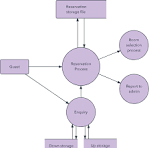
\includegraphics{Pictures/save.png}
You should follow the divide and conquer theory, so divide the overall problem into more manageable parts and develop each part or module separately. When all modules are ready, you should integrate all the modules into one system. In this phase, you should briefly describe all the modules and the functionality of these modules.
\textbf{Elements of Project Development}

\section{Data Design}
Data design will consist of how you organize, managing and manipulate the data.

\textit{Schema Design: Define the structure and explanation of schemas used in your project.}

\textit{Data Integrity and Constraints: Define and explain all the validity checks and constraints you are providing to maintain data integrity.}

\subsection{Schema Design}

\subsection{Data Integrity and Constraints}

\section{Procedural Design}
Procedural design is a systematic way for developing algorithms or procedurals.

\textit{Logic Diagrams: Define the systematical flow of procedure that improves its comprehension and helps the programmer during implementation. e.g., Control Flow Chart, Process Diagrams etc.}

\textit{Data Structures: Create and define the data structure used in your procedures.}

\textit{Algorithms Design: With proper explanations of input data, output data, logic of processes, design and explain the working of algorithms.}

\subsection{Logic Diagrams}

\subsection{Data Structures}

\subsection{Algorithms Design}

\section{User interface design}
Define user, task, environment analysis and how you intend to map those requirements in order to develop a “User Interface”. Describe the external and internal components and the architecture of your user interface. Show some rough pictorial views of the user interface and its components.

\section{Security Issues}
Discuss Real-time considerations and Security issues related to your project and explain how you intend avoiding those security problems. What are your security policy plans and architecture?

\section{Test Cases Design}
Define test cases, which will provide easy detection of errors and mistakes with in a minimum period of time and with the least effort. Explain the different conditions in which you wish to ensure the correct working of your software. 
%% Chapter Template

\chapter{IMPLEMENTATION AND TESTING} % Main chapter title

\label{Chapter5} % Change X to a consecutive number; for referencing this chapter elsewhere, use \ref{ChapterX}

\lhead{Chapter 5. \emph{IMPLEMENTATION AND TESTING}} % Change X to a consecutive number; this is for the header on each page - perhaps a shortened title

%----------------------------------------------------------------------------------------
%	SECTION 1
%----------------------------------------------------------------------------------------

\section{Implementation Approaches}
Define the plan of implementation, and the standards you have used in the implementation.
\section{Coding Details and Code Efficiency}
Students not need include full source code, instead, include only the important codes (algorithms, applets code, forms code etc).The program code should contain comments needed for explaining the work a piece of code does. Comments may be needed to explain why it does it, or, why it does a particular way. You can explain the function of the code with a shot of the output screen of that program code.

\textit{Code Efficiency: You should explain how your code is efficient and how you have handled code optimisation.}

\subsection{Code Efficiency}

\section{Testing Approach}
Testing should be according to the scheme presented in the system design chapter and should follow some suitable model – e.g., category partition, state machine-based. Both functional testing and user-acceptance testing are appropriate. Explain your approach of testing.

\textbf{Project Structure}

\textit{Unit Testing: Unit testing deals with testing a unit or module as a whole. This would test the interaction of many functions but, do confine the test within one module.}

\textit{Integrated Testing: Brings all the modules together into a special testing environment, then checks for errors, bugs and interoperability. It deals with tests for the entire application. Application limits and features are tested here.}

\subsection{Unit Testing}

\subsection{Integrated Testing}

\section{Modifications and Improvements}
Once you finish the testing you are bound to be faced with bugs, errors and you will need to modify your source code to improve the system. Define what modification you implemented in the system and how it improved your system.
 
%% Chapter Template

\chapter{RESULTS AND DISCUSSION} % Main chapter title

\label{Chapter6} % Change X to a consecutive number; for referencing this chapter elsewhere, use \ref{ChapterX}

\lhead{Chapter 6. \emph{RESULTS AND DISCUSSION}} % Change X to a consecutive number; this is for the header on each page - perhaps a shortened title

%----------------------------------------------------------------------------------------
%	SECTION 1
%----------------------------------------------------------------------------------------

\section{Test Reports}
Explain the test results and reports based on your test cases, which should show that your software is capable of facing any problematic situation and that it works fine in different conditions. Take the different sample inputs and show the outputs.

\section{User Documentation}
Define the working of the software; explain its different functions, components with screen shots. The user document should provide all the details of your product in such a way that any user reading the manual is able to understand the working and functionality of the document.

 
%\input{Chapters/Chapter7} 

%----------------------------------------------------------------------------------------
%	THESIS CONTENT - APPENDICES
%----------------------------------------------------------------------------------------

\addtocontents{toc}{\vspace{2em}} % Add a gap in the Contents, for aesthetics

\appendix % Cue to tell LaTeX that the following 'chapters' are Appendices

% Include the appendices of the thesis as separate files from the Appendices folder
% Uncomment the lines as you write the Appendices

% Appendix Template

\chapter{Appendix A} % Main appendix title

\label{AppendixA} % Change X to a consecutive letter; for referencing this appendix elsewhere, use \ref{AppendixX}

\lhead{Appendix A. \emph{Appendix Title Here}} % Change X to a consecutive letter; this is for the header on each page - perhaps a shortened title

Write your Appendix content here.....These may be provided to include further details of results, mathematical derivations, certain illustrative parts of the program code (e.g., class interfaces), user documentation etc.

\textbf{\Large PROJECT REPORT STRUCTURE}

\textbf{INTRODUCTION}

The project report should be documented with an engineering approach to the solution of the problem that you have sought to address. The project report should be prepared in order to solve the problem in a methodical and professional manner, making due references to appropriate techniques, technologies and professional standards. You should start the documentation process from the first step of software development so that you can easily identify the issues to be focused upon in the ultimate project report. You should also include the details from your project notebook, in which you would have recorded the progress of your project throughout the course. The project report should contain enough details to enable examiners to evaluate your work. The
details, however, should not render your project report as boring and tedious. The important points should be highlighted in the body of the report, with details often
relegated to appendices

\textbf{IMPORTANCE OF PROJECT/PROJECT REPORT}

The Mini Project is not only a part of the coursework, but also a mechanism to demonstrate your abilities and specialisation. It provides the opportunity for you to demonstrate originality, teamwork, inspiration, planning and organisation in a software project, and to put into practice some of the techniques you have been taught throughout the previous courses. The Mini Project is important for a number of reasons. It provides students with:

\begin{enumerate}
\item[$\bullet$]opportunity to specialise in specific areas of IT;
\item[$\bullet$]future employers will most likely ask you about your project at interview;
\item[$\bullet$]opportunity to demonstrate a wide range of skills and knowledge learned, and
\item[$\bullet$]encourages integration of knowledge gained in the previous course units.
\end{enumerate}


\textbf{The project report is an extremely important aspect of the project. It serves to show what you have achieved and should demonstrate that:}

\textbf{\textit{Elements of Project Development}}
\begin{enumerate}


\item[$\bullet$]You understand the wider context of computing by relating your choice of the
project, and the approach you take, to existing products or research.

\item[$\bullet$]You can apply the theoretical and practical techniques taught in the course to
the problem you are addressing and that you understand their relevance to the
wider world of computing.

\item[$\bullet$]You are capable of objectively criticising your own work and making constructive suggestions for improvements or further work based on your experiences so far.

\item[$\bullet$]You can explain your thinking and working processes clearly and concisely to others through your project report.

\end{enumerate}

%
%\input{Appendices/AppendixC}

\addtocontents{toc}{\vspace{2em}} % Add a gap in the Contents, for aesthetics

\backmatter

%----------------------------------------------------------------------------------------
%	BIBLIOGRAPHY
%----------------------------------------------------------------------------------------
\nocite{*}
\label{Bibliography}

\lhead{\emph{Bibliography}} % Change the page header to say "Bibliography"

\bibliographystyle{apalike} % Use the "custom" BibTeX style for formatting the Bibliography

%\bibliographystyle{unsrt}

\bibliography{Bibliography} % The references (bibliography) information are stored in the file named "Bibliography.bib"

\end{document}  








\documentclass{report}
\usepackage{fancyhdr,graphicx}
\usepackage{lipsum}


\begin{document}
\fancyhf{}% Clear fancy header/footer
\fancyhead[L]{\raisebox{-1.0\height}[0pt][0pt]{
\includegraphics[scale=0.15]{Pictures/KGCE_Letter_head_header.png}}}
\fancyhead[R]{\leftmark}
\pagestyle{fancy}

\chapter{A chapter}


\end{document}

